%%%%%%%%%%%%%%%%%%%%%%%%%%%%%%%%%%%%%%%%%%%%%%%%%%%%%%%%
% Created by Pierre Chardaire. Updated by Rudy Lapeer
% Last update: 10/2024
% Change the option between square brackets
% depending on the document you have to write:
%
% review      for the literature review + plan
% progress    for the progress report
% final       for the final report
% 
%%%%%%%%%%%%%%%%%%%%%%%%%%%%%%%%%%%%%%%%%%%%%%%%%%%%%%%%
\documentclass[review]{cmpreport}


% Some package I am using. You may not need them
%
\usepackage{rotating}
\usepackage{subfloat}
\usepackage{color}
\usepackage{pdfpages}

%\setkeys{Gin}{draft}

%%%%%%%%%%%%%%%%%%%%%%%%%%%%%%%%%%%%%%%%%%%%%%%%%%%%%%%%
%
%  Fill in the fields with:
%
%  your project title
%  your name
%  your registration number
%  your supervisor's name
%
%%%%%%%%%%%%%%%%%%%%%%%%%%%%%%%%%%%%%%%%%%%%%%%%%%%%%%%%
\title{Agri Robot Mapping and Pathing Literature Review}
%%%%%%%%%%%%%%%%%%%%%%%%%%%%%%%%%%%%%%%%%%%%%%%%%%%%%%%%
%
% The author's name is ignored if the following command 
% is not present in the document
%
% Before submitting a PDF of your final report to the 
% project database you may comment out the command
% if you are worried about lack of anonymity.
%
%%%%%%%%%%%%%%%%%%%%%%%%%%%%%%%%%%%%%%%%%%%%%%%%%%%%%%%%
\author{Toby Towler}

\registration{Your registration}
\supervisor{Edwin Ren}

%%%%%%%%%%%%%%%%%%%%%%%%%%%%%%%%%%%%%%%%%%%%%%%%%%%%%%%%
%
% Fill in the field with your module code.
% this should be:
%
% for BIS project module   -> CMP-6012Y
% for STATS project module -> CMP-6028Y
% for CS project module    -> CMP-6013Y
%
%%%%%%%%%%%%%%%%%%%%%%%%%%%%%%%%%%%%%%%%%%%%%%%%%%%%%%%%
\ccode{CMP-6013Y}

%%%%%%%%%%%%%%%%%%%%%%%%%%%%%%%%%%%%%%%%%%%%%%%%%%%%%%%%
%
% Comment out if confidential report.
% The command should be used if the project is subjected 
% to a Non Disclosure Agreement.
%
% Three examples of the use of the \confidential command. 
% Please ask your supervisor what confidential statement 
% should be used, if appropriate.
%
%%%%%%%%%%%%%%%%%%%%%%%%%%%%%%%%%%%%%%%%%%%%%%%%%%%%%%%%
%\confidential{}

%\confidential{The contents of this report remain confidential for two years and should not be discussed or disclosed to any third party without the prior written permission from the School of Computing Sciences, the University of East Anglia}

%\confidential{The information contained in this document is confidential, privileged and only for the information of the intended recipient and may not be used, published or redistributed without the prior written consent of FruitName Ltd}

\summary{
This document explains how to use the class file \texttt{cmpreport.cls} to write your reports.
The class file has been designed to simplify your life; many things are done for you. As a consequence
some commands presented here are specific to the class file whether they are new commands or customized versions
of commonly known \LaTeX\ commands.
}

\acknowledgements{
This section is used to acknowledge whoever's support and contribution.
The command that introduces it is ignored in the project literature review and progress report. It is used in the final report,  but  is not compulsory. If you do not
have an acknowledgements command in your preamble then there
won't be any acknowledgement section in the document produced. \emph{Abstract} and \emph{Acknowledgements} sections should fit on the same page. 
}

%%%%%%%%%%%%%%%%%%%%%%%%%%%%%%%%%%%%%%%%%%%%%%%%%%%%%%%%%%%%%%%%%%
%
% If you do not want a list of figures and a list of tables
% to appear after the table of content then uncomment this line 
%
% Note that the class file contains code to avoid
% producing an empty list section (e.g list of figures) if the 
% list is empty (i.e. no figure in document).
%
% The command also prevents inserting a list of figures or tables 
% anywhere else in the document
%
% Some supervisors think that a report should not contain these
% lists. Please ask your supervisor's opinion.
%
%%%%%%%%%%%%%%%%%%%%%%%%%%%%%%%%%%%%%%%%%%%%%%%%%%%%%%%%%%%%%%%%%%
%\nolist

%%%%%%%%%%%%%%%%%%%%%%%%%%%%%%%%%%%%%%%%%%%%%%%%%%%%%%%%%%%%%%%%%%
%
% Comment out if you want your list of figures and list of
% tables on two or more pages, in particular if the lists do not fit 
% on a single page.
%
%%%%%%%%%%%%%%%%%%%%%%%%%%%%%%%%%%%%%%%%%%%%%%%%%%%%%%%%%%%%%%%%%%
\onePageLists


\begin{document}


\section{Introduction}

Before reading this document you should go through the \LaTeX\ tutorials that have been provided for you to learn the basics of \LaTeX\ such as sectioning, style, lists, referencing, bibliography and mathematics if applicable.
Even if you already  know \LaTeX{}, please at least go through \emph{Tutorial 6: Bibliography and citations in \LaTeXe{}} and \emph{Tutorial 5: Producing professional-looking tables}.

%\interfootnotelinepenalty=10000
The basic structure of your reports is introduced in section~\ref{sec1} with the \LaTeX{} commands used to implement it\footnote{The beginning of your reports, usually the \emph{Introduction} section, should tell the reader about the organisation of the report.}. Section~\ref{sec2} shows how to create figures and gives examples of tables produced with the \verb/cmpreport/ class. Section~\ref{secGantt} shows how you can produce a Gantt chart with \LaTeXe{}. 

\section{The structure of the document} \label{sec1}

As any other \LaTeX{} documents, your report starts by declaring the style of your document. For your final report this is done by issuing the command 
\texttt{\textbackslash{}documentclass\allowbreak [final]\{cmpreport\}}
which means that your report follows the style specified for the \texttt{final} report in the file \texttt{cmpreport.cls}. Your bibliography file (\verb/bib/ file) and any pictures you use in your figures should be placed in the same directory as your report. The option \texttt{final}, between the square brackets, must be replaced with \texttt{review} or \texttt{progress} for the corresponding pieces of assessment.
There is another option \texttt{tutorial} that you will have used if you went through some of my tutorials. However, this is of no concern when using the class for your reports.

The main differences between the options of interest are:
\begin{itemize}
\item The option \texttt{review} produces a simple title page and add a ``performance sheet''\footnote{This is not a mark sheet, as this corresponds to a formative piece of coursework. However, your supervisor may indicate a level of performance for each of the criteria in the performance sheet.} at the end of the document that indicates the evaluation criteria
for the corresponding piece of work and provides a comment box for your supervisor. 
\item The option \texttt{final} provides a ``more official'' title page\footnote{You may want to show your report to a future employer.}. It creates a table of contents, and possibly a list of tables and a list of figures (see below). 
\end{itemize}

\subsection{The preamble}

The structure of your document preamble is as follows:
\begin{verbatim}
\documentclass[final]{cmpreport}
\title{A simple proof that $P \ne NP$}
\author{Harold P\'etard}
\registration{31415927}
\supervisor{Dr Ersatz Stanislaus Pondiczery}
\ccode{CMP-6012Y}
%\confidential{}
\summary{This document shows that $P \ne NP$.}
\acknowledgements{
I would like to thank my supervisor Dr Ersatz 
Stanislaus Pondiczery, from the Royal Institute of 
Poldavia, for observing that the fundamental 
difference between $P$ and $NP$ is the letter $N$.
}
%\nolist
\onePageLists
\end{verbatim}
The \LaTeX{} source of this document contains extra comments to explain these commands.

If the command \verb/\author/ is present the name provided will appear as author of the report. The command \verb/\author/ is not compulsory because, at some point, you'll have  to submit an electronic  version of your final report to a School database that future students can consult. You may not want your name to appear in the electronic version. It is up to you, \emph{but do not forget to use the} \verb/\author/ \emph{command to produce printed versions}.

\verb/\registration/, \verb/\supervisor/ and \verb/\ccode/ are all compulsory for all reports. \verb/\summary/ and \verb/\acknowledgements/ produce the \emph{Abstract} and \emph{Acknowledgements} sections. These two commands are for the final report; the first one is compulsory, the second one, optional.

In the final report, a \emph{List of figures} followed by a \emph{List of tables} are automatically constructed after the \emph{Contents} section. The \verb/cmpreport/ class is intelligent enough to realise that any such list should not be created if nothing goes in that list, that is if you do not have figures or do not have tables in your document. In addition, use the command \verb/\onePageLists/ if you have modest-size lists you want to fit on a single page.

Some supervisors are of the opinion that list of tables and list of figures should not be included in a report. If this is the case you just have to uncomment the command \verb/\nolist/\footnote{Reminder: By now you should know that anything that follows a \% is a comment.}. This also blocks the use of the standard \LaTeXe{} commands for creating list of figures and list of tables. 

The command \verb/\confidential{}/ adds a confidential stamp to the margin of each page. This should only be used in specific cases that in general involve a non-disclosure agreement.

Note that \LaTeX{} truncates the progress report if it exceeds twenty-two pages and the final report if it exceeds fifty-five pages as limits in the number of pages are requirement for these deliverables\footnote{The truncation values are ten percent over the requirement limits to comply with University regulations.\newline To be clear the limit for the final report is 50 pages, meaning up to 55 pages will be accepted.}.

\subsection{Your document}

The structure of your document (after the preamble) should be of the form

\begin{verbatim}
\begin{document}
% Main content of report goes here
\clearpage
\bibliography{reportbib}
\clearpage
\appendix
\section{My first appendix}
% content of first appendix
\clearpage
\section{My second appendix}
% content of second appendix
\end{document}
\end{verbatim}

You should not need to use the command \verb/\maketitle/. Making the title is compulsory and is taken care of by the \texttt{cmpreport} class.

\section{Producing tables and figures} \label{sec2}

Tables are produced using a rewriting of the table environment that is specific to the report class. This new environment \verb/cmptable/ imposes some choices onto the user of the class to ensure a particular style in the report, but also provides new commands to facilitate the writing of quality tables. Tables \ref{table2} and \ref{table3} show examples of tables produced using this environment. Details are provided in \citet{PCtut5}. 

\begin{cmptable}[h]
	{Rates of DHS\tnote{a} shelter use by selected characteristics\label{table2}}
	\begin{tabular}{L{0.05}L{0.35}SSS} 
		\toprule
		&& \mcc[3]{Shelter system}\\ \cmidrule{3-5}
		
		&&  \mcc(0.20){Either\tnote{b}\newline (\%)} 
		&   \mcc(0.20){Family\newline (\%)}
		&   \mcc(0.20){Single Adult\newline (\%)} \\ \uhrule
		
		\mcl[2]{\emph{History of out-of-home care:}} \\ 
		& Yes & 22.4 & 17.0 & 8.9 \\
		& No  & 10.8 &  9.4 & 2.5 \\ \addlinespace
		
		
		\mcl[2]{\emph{Type of final exit from ACS\mtnote{c}:}} \\
		&  Reunification       & 19.4 & 14.7 & 7.6 \\
		& Independent living   & 25.6 & 18.8 & 10.7 \\
		& Absconding from care & 33.6 & 22.4 & 15.6 \\
		& Preventive services  & 12.4 & 11.0 & 3.0 \\ \addlinespace
		
		\bottomrule
	\end{tabular}
	\begin{tablenotes}
		\item[a] Department of Homeless Services.
		\item[b] This category reflects the unduplicated sum of the other two columns.
		\item[c] The New-York City Administration for Children's Services.
		\note{All relationships are statistically significant for $\chi^2$ test ($p<.001$).}
		\note{Source: \cite{UCP}.} %This is a general note
	\end{tablenotes}
\end{cmptable}

\begin{cmptable}[h]
	{Effect of parameters on performance\tnote{a}\label{table3}}
	\begin{tabular}{S[
			table-format=6, 
			table-space-text-post = \mtnote{b}]
			SSSS}
		\toprule
		\mcc(0.3){Parameter} & \mcc[4]{Data set} \\ \cmidrule{2-5}
		& \mcc[2]{\textsc{Single}} & \mcc[2]{\textsc{Multiple}} \\ \cmidrule[r]{2-3} \cmidrule[l]{4-5}
		& \mcc(0.175){CPU \newline (msec)} 
		& \mcc(0.175){Effective\newline (\%)} 
		& \mcc(0.175){CPU\newline (msec)} 
		& \mcc(0.175){Effective\newline (\%)} \\ \uhrule
		
		\mcc{$n (k=10, p=100)$} \\
		2 & 75.5 & 55.5 & 174.2 & 22.2 \\
		3 & 21.5 & 50.4 &  79.4 & 19.9 \\
		4 & 16.9 & 47.5 &  66.1 & 16.3 \\ \midrule
		
		\mcc{$k (n=2, p=100)$} \\
		10   &  57.5 & 51.3 & 171.4 & 21.7 \\
		100  &  60.0 & 56.1 & 163.1 & 21.3 \\
		1000 & 111.3 & 55.9 & 228.8 & 21.4 \\ \midrule
		
		\mcc{$p (n=2, k=10)$} \\
		100      &  3.3 &  5.5 &   6.1 &  1.2\\ 
		1000     & 13.8 & 12.6 &  19.8 &  2.1 \\
		10000    & 84.5 & 56.0 & 126.4 &  6.3 \\
		100000 \mtnote{b}  & \mcc{---}  & \mcc{---}  & 290.7 & 21.8 \\
		\bottomrule
	\end{tabular}
	\begin{tablenotes}
		\item[a] Results on processing time and effectiveness for
		various combinations of the three parameters for both data sets. Default parameters are shown in parentheses.
		\item[b] Value not meaningful for the data set {\textsc{Single}}.
		\note{Adapted from \cite{zobel}.}
	\end{tablenotes}
\end{cmptable}
\clearpage
The figure environment has also been rewritten so that the caption is now a compulsory parameter of the environment. 
Note that the \verb/label/ command for the figure must be included just before the closing brace of the caption parameter.
The code:
\begin{verbatim}
\begin{cmpfigure}[htb]{Cool cat \label{fig1}}
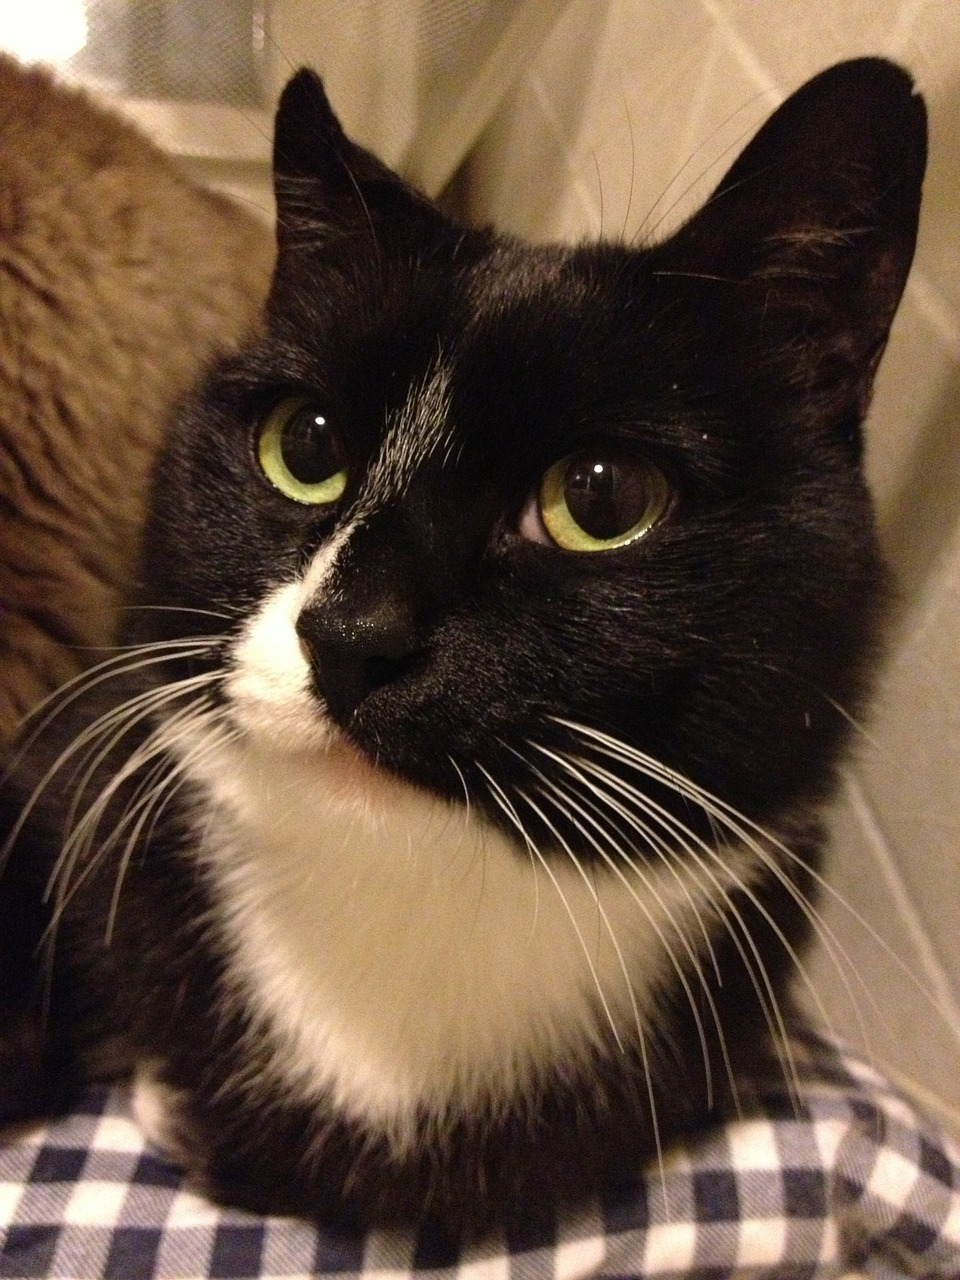
\includegraphics[width=0.5\textwidth]{coolcat.jpg}
\begin{tablenotes}
\item Image in the public domain.
\end{tablenotes}
\end{cmpfigure}
\end{verbatim}
produces figure~\ref{fig1}.

\begin{cmpfigure}[htb]{Cool cat \label{fig1}}
	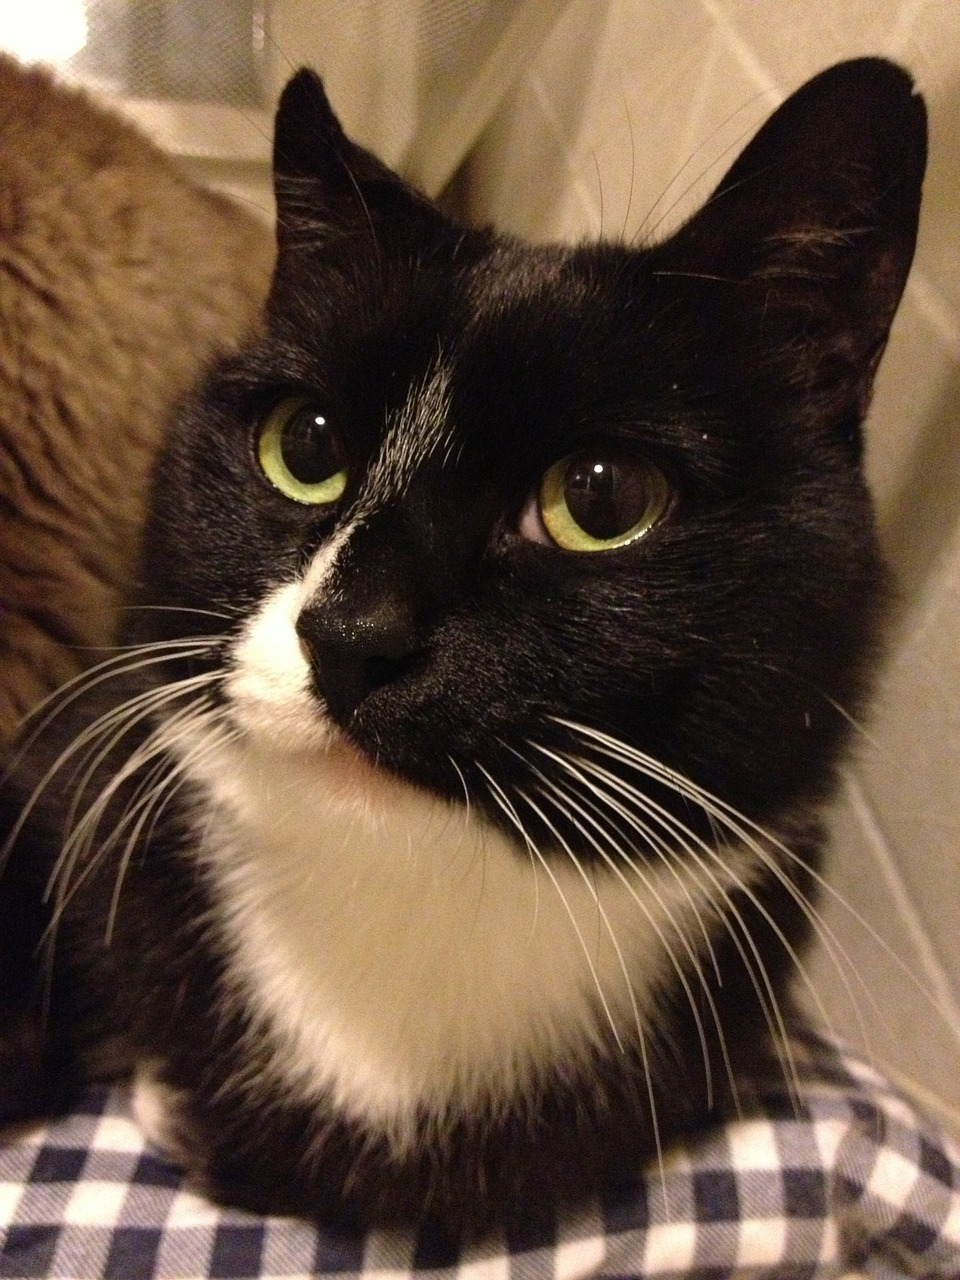
\includegraphics[width=0.3\textwidth]{coolcat.jpg}
	\begin{tablenotes}
		\item Image in the public domain.
	\end{tablenotes}
\end{cmpfigure}

Figures, as tables, should \textbf{not} be centred.  Figure~\ref{fig2}, whose code is given in Appendix~\ref{ApA}, shows an example of a figure that includes sub-figures. The choice of parameters in the code was slightly complicated by the fact that I used photographs that I did not crop to size. Only a few students working on Graphics projects may need sub-figures. The sub-figures can be referenced: the command \verb/\ref{fig2:tired}/ produces ``\ref{fig2:tired}''

\begin{cmpfigure}[ht!p]{Cats \label{fig2}}
         \begin{subfigure}[b]{0.2\textwidth}
                 \centering
                 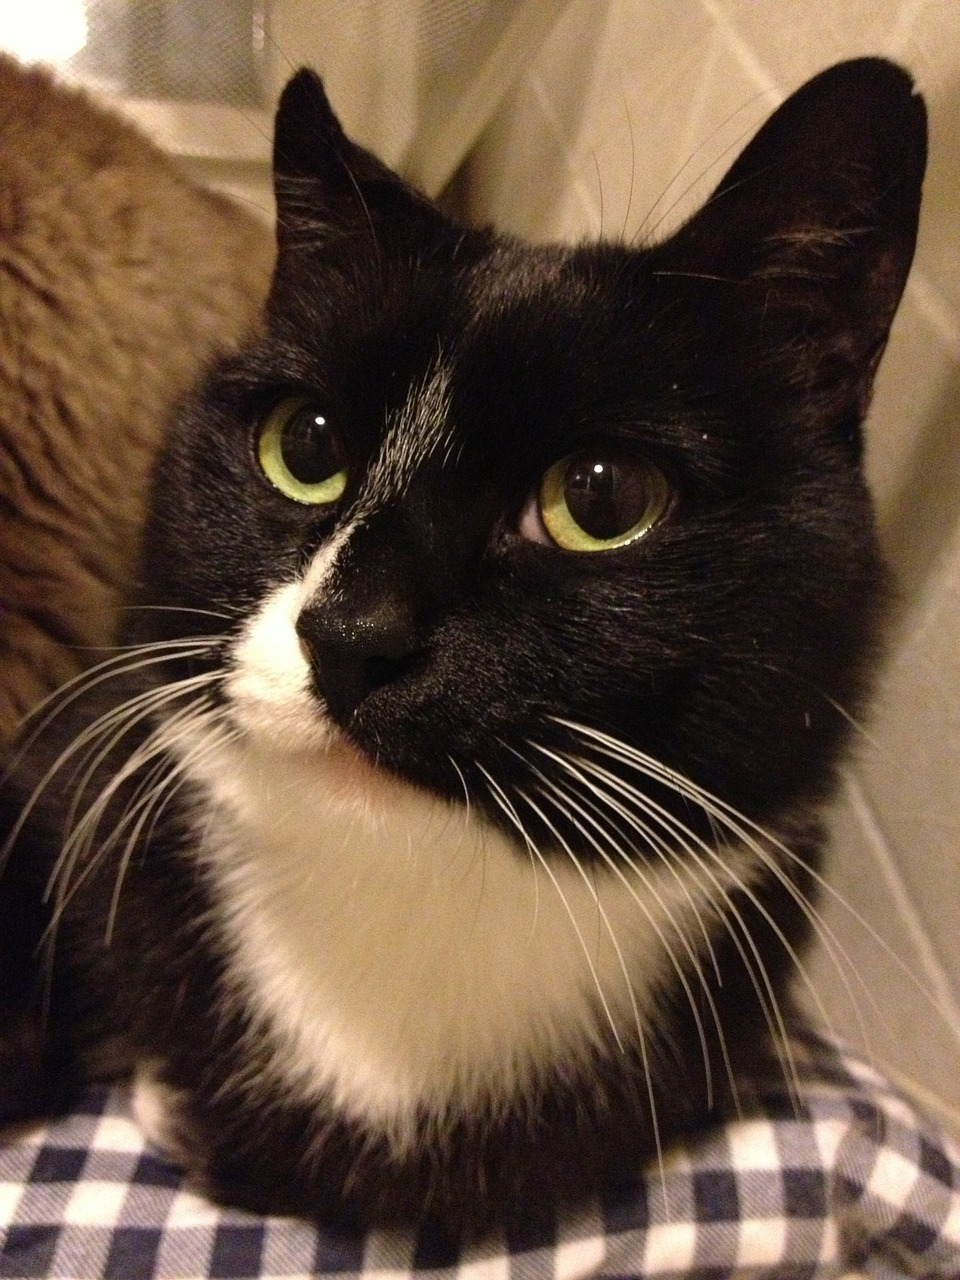
\includegraphics[width=0.98\textwidth]{coolcat}
                 \caption{Cool}
                 \label{fig2:coolcat}
         \end{subfigure}
         \begin{subfigure}[b]{0.398\textwidth}
                 \centering
                 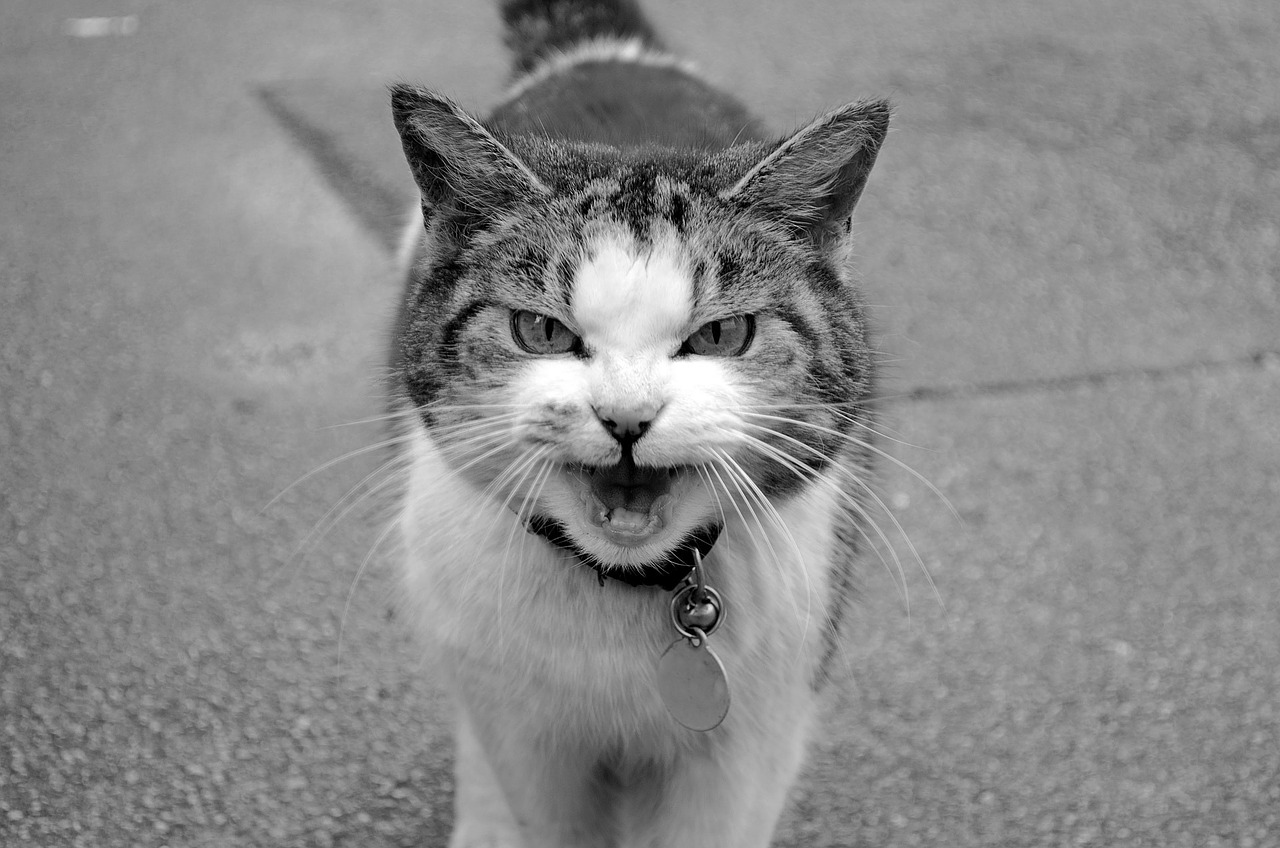
\includegraphics[width=0.99\textwidth]{bossycat}
                 \caption{Bossy}
                 \label{fig2:bossycat}
         \end{subfigure}%
         \begin{subfigure}[b]{0.4\textwidth}
                 \flushright
                 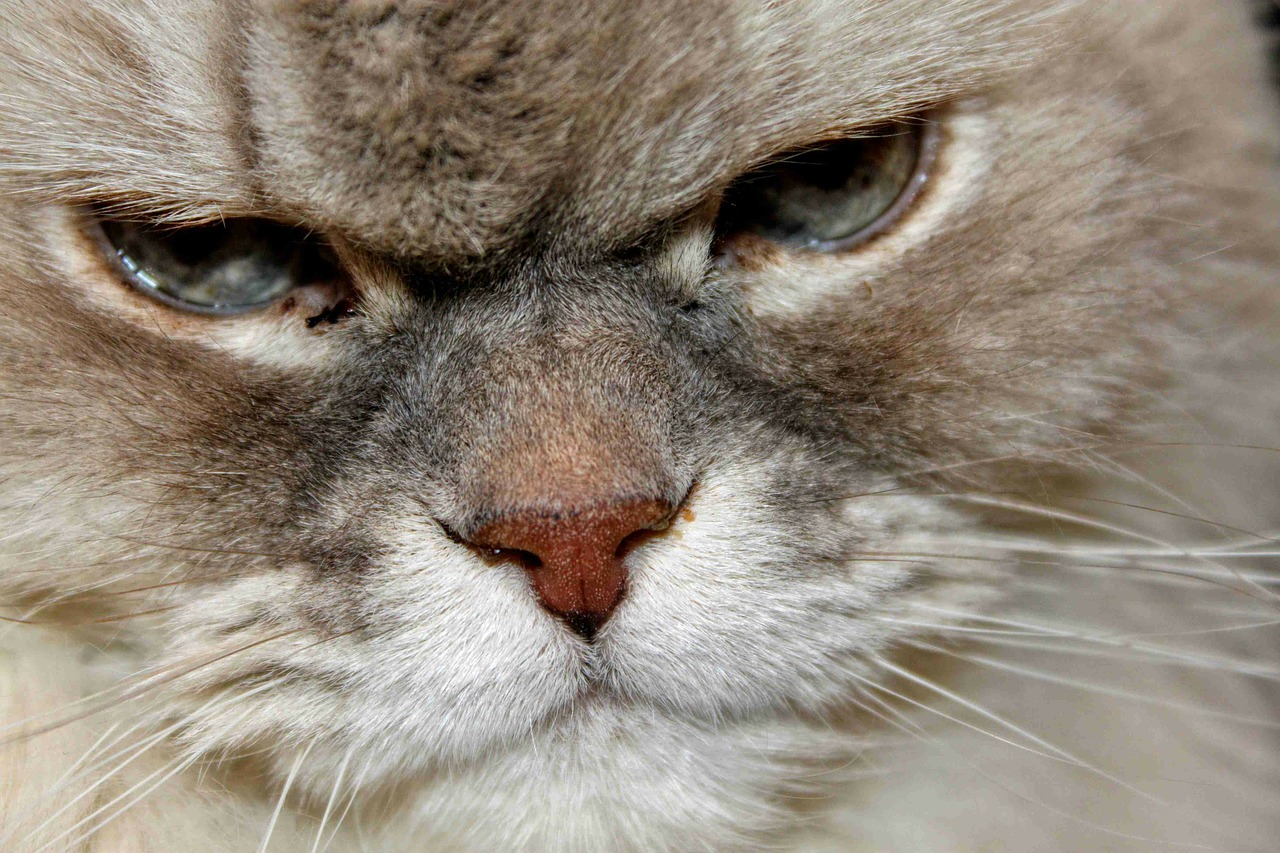
\includegraphics[width=0.98\textwidth]{frowningcat}
                 \caption{Reflective}
                 \label{fig2:frowningcat}
         \end{subfigure}
% leave a blank line to change row         
         
         \begin{subfigure}[b]{0.31\textwidth}
                 \centering
                 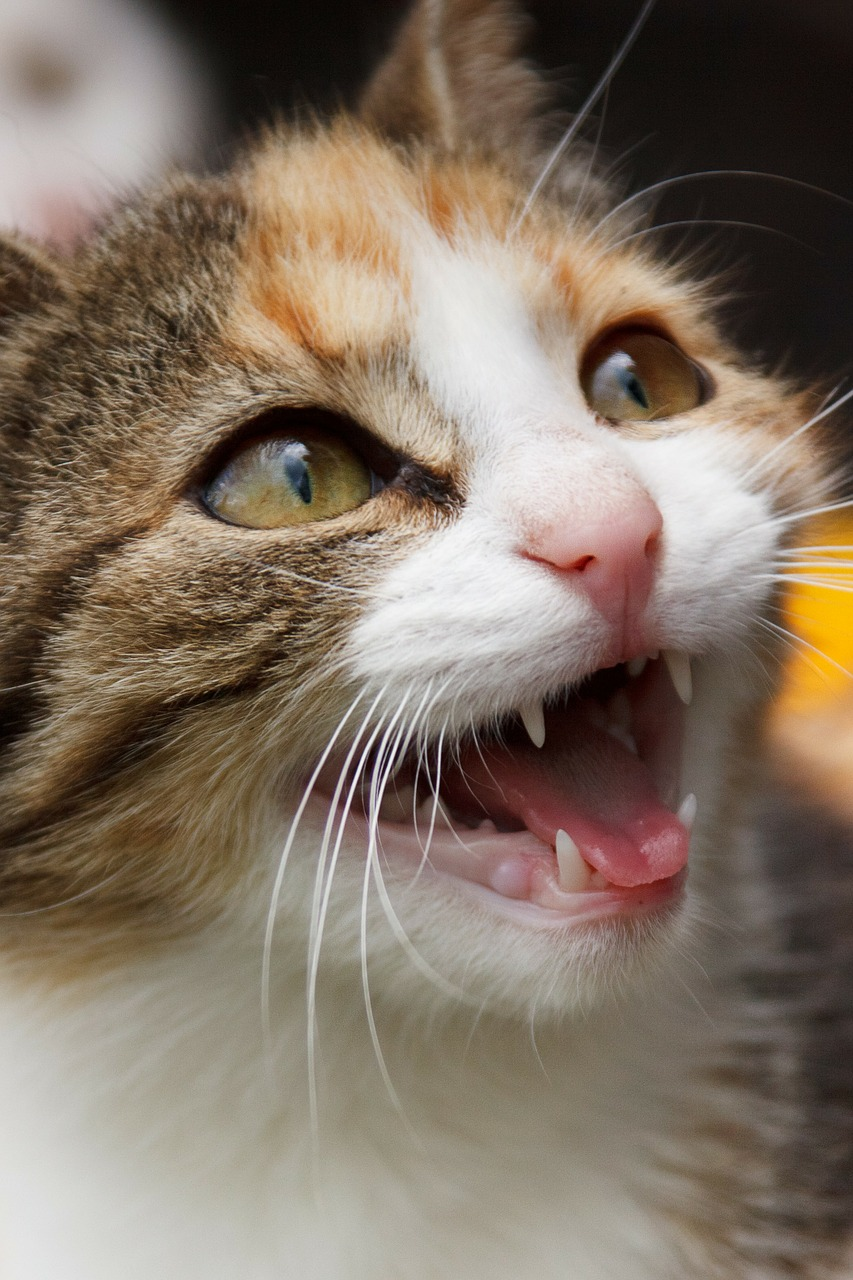
\includegraphics[width=0.985\textwidth]{scaredbabycat}
                 \caption{Scared}
                 \label{fig2:scared}
         \end{subfigure}
         \begin{subfigure}[b]{0.69\textwidth}
                 \centering
                 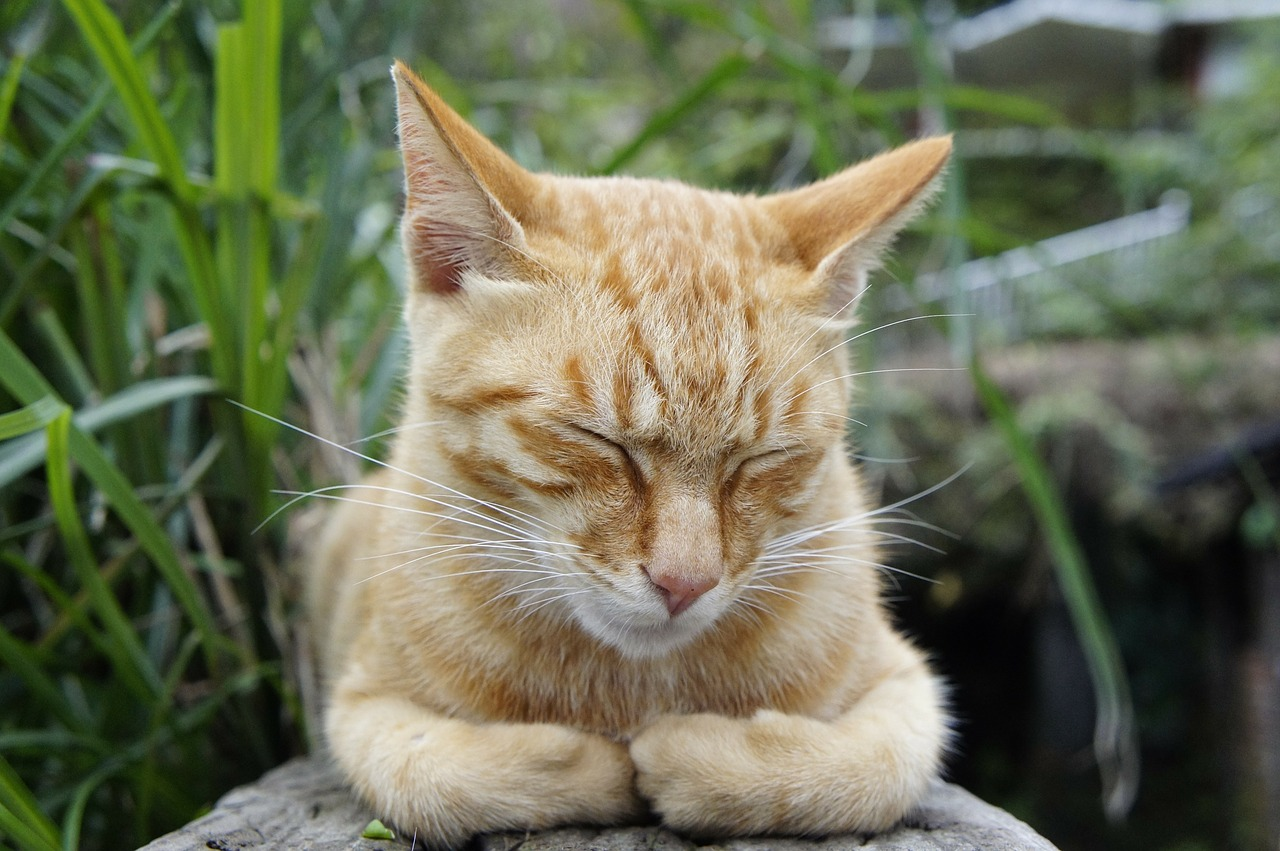
\includegraphics[width=\textwidth]{tiredcat}
                 \caption{Tired}
                 \label{fig2:tired}
         \end{subfigure}
\begin{tablenotes}
\item Images in the public domain.
\end{tablenotes}
\end{cmpfigure}

\section{Producing a Gantt chart}\label{secGantt}

The Gantt chart in figure~\ref{pplan} is produced by the code in figure~\ref{codepplan} and can be found in Appendix~\ref{ApB}. To compile this code you need to include the command \verb|\usepackage{rotating}| in your preamble.  

You may want to reuse this code and only modify the part that starts with the elements, bars and milestones, as the granularity of the schedule is right. The commands used in this part are as follows
\begin{itemize}
\item \verb|\ganttbar{Final report writing}{25}{30}| creates a task named \texttt{Final report writing} and an associated bar that goes from the 25th time slot of the schedule to the 30th.
\item \verb|\ganttvoidbar{}{13}{16}| creates a grey bar from the 13th slot to the 16th to show a period of break in a task.
\item \verb|\ganttmilestone{Code delivery}{26}| shows a milestone in the 26th slot.
\item \verb|\\| indicates a change of line in the schedule. Notice how three bars without change of lines are used to show the tasks that include a break period in grey.
\item \verb|\ganttlink{elem0}{elem2}| creates a link from \texttt{elem0} to \texttt{elem2}. \texttt{elem0, elem1,\ldots} are identifiers of the bars and milestones in the order they are introduced in the code. 
\end{itemize}

\begin{cmpfigure}{Code for the Gantt chart of Figure~\ref{pplan}\label{codepplan}}
{\scriptsize
\begin{verbatim}
\begin{cmpfigure}{Project Gantt chart \label{pplan}}
\begin{sideways}
\newganttchartelement{voidbar}{
voidbar/.style={
draw=black,
top color=black!25,
bottom color=black!23
}}
\begin{ganttchart}[x unit=0.35cm, y unit chart = 1.0cm, 
y unit title=0.5cm, title height=1.0, vgrid, 
title label font=\scriptsize,
canvas/.style={draw=black, dotted},
/pgfgantt/milestone left shift = 0,
/pgfgantt/milestone right shift = 0
]{1}{34}
\gantttitle{Project schedule shown for semester week numbers}{34} \\
\gantttitlelist{1,...,34}{1}\\
\gantttitlelist{1,...,12}{1}
\gantttitle{CB}{4}
\gantttitle{AP}{2}
\gantttitlelist{1,...,8}{1}
\gantttitle{EB}{4}
\gantttitlelist{9,...,12}{1}\\

%the elements, bars and milestones, are identified as elem0, elem1, etc.

%elem1
\ganttbar{Project proposal}{1}{2}          \\     %elem0  
\ganttbar{Literature review}{2}{5}         \\     %elem1 
\ganttbar{Design}{6}{11}                   \\     %elem2

%week 1 of semester 2 is the 17th week in schedule 
\ganttbar{Coding}{12}{12}                         %elem3
\ganttvoidbar{}{13}{16}                           %elem4
\ganttbar{}{17}{20}                        \\     %elem5

\ganttbar{Testing}{12}{12}                        %elem6
\ganttvoidbar{}{13}{16}                           %elem7
\ganttbar{}{17}{26}                        \\     %elem8
\ganttmilestone{Code delivery}{26}         \\     %elem9
\ganttbar{Final report writing}{25}{30}    \\     %elem10
\ganttmilestone{Portfolio submission}{33}  \\     %elem11
\ganttbar{Inspection preparation}{31}{34}         %elem12

\ganttlink{elem0}{elem2} \ganttlink{elem1}{elem2} \ganttlink{elem2}{elem3}
\ganttlink[link mid=.25]{elem2}{elem6} \ganttlink{elem5}{elem6}
\ganttlink{elem8}{elem9} \ganttlink{elem9}{elem10}
\ganttlink{elem10}{elem11} \ganttlink{elem11}{elem12}
\end{ganttchart}
\end{sideways}
\end{cmpfigure}
\end{verbatim}
}
\end{cmpfigure}

\section{Producing an appendix}

To create an appendix, make sure you use the \verb|\appendix| command to make sure that subsequent \verb|\section{}| commands will be labelled "Appendix X" rather than carrying on with text body section numbers (e.g Section 6). 
\clearpage

\bibliography{reportbib}

\appendix
\clearpage
\section{Code for the ``Cats'' figure} \label{ApA}
\enlargethispage{10\baselineskip}
{\footnotesize
\begin{verbatim}
\begin{cmpfigure}[htp]{Cats \label{fig2}}
         \begin{subfigure}[b]{0.2\textwidth}
                 \centering
                 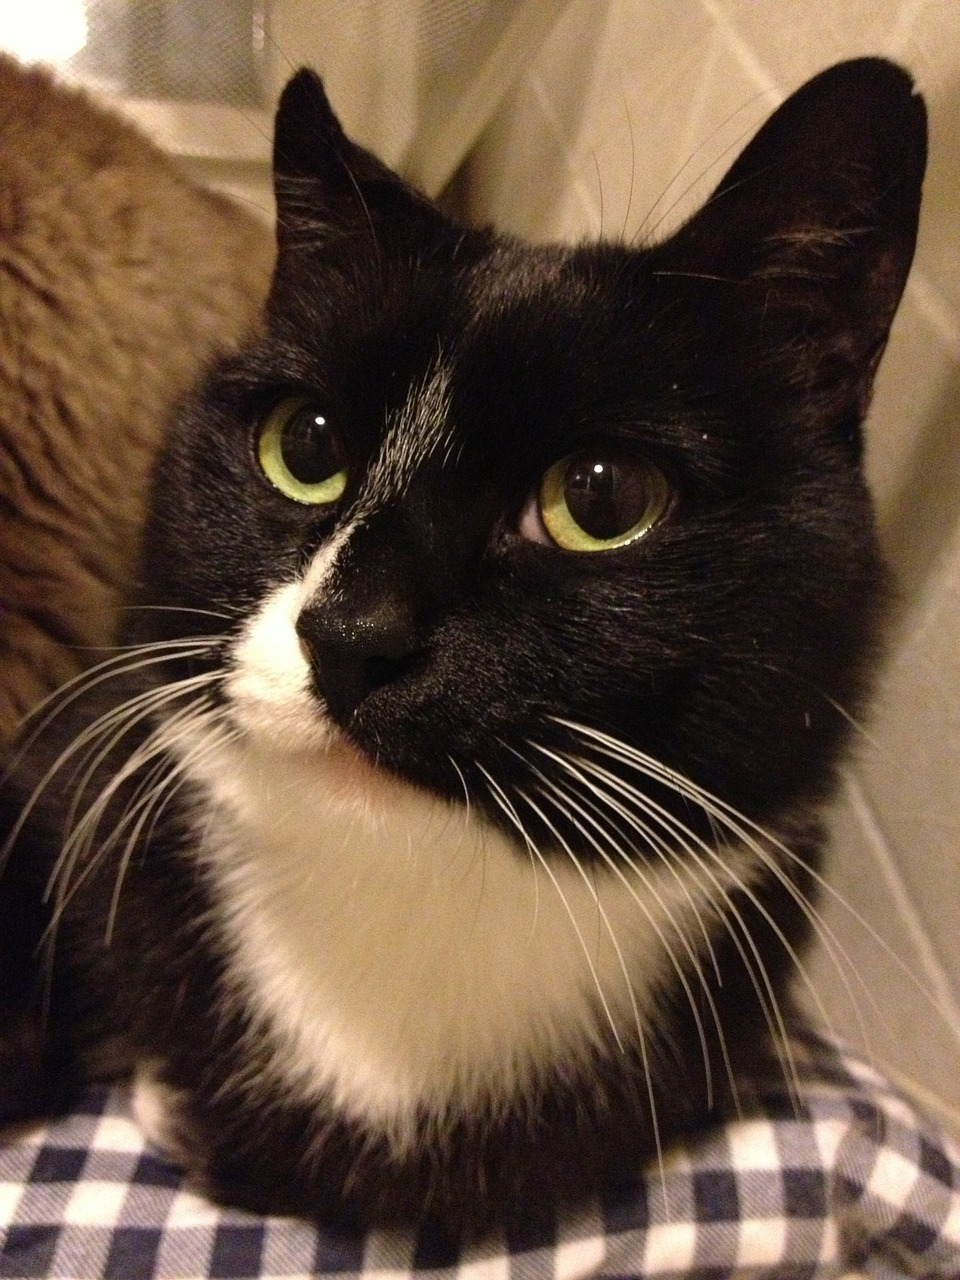
\includegraphics[width=0.98\textwidth]{coolcat}
                 \caption{Cool} \label{fig2:coolcat}
         \end{subfigure}
         \begin{subfigure}[b]{0.398\textwidth}
                 \centering
                 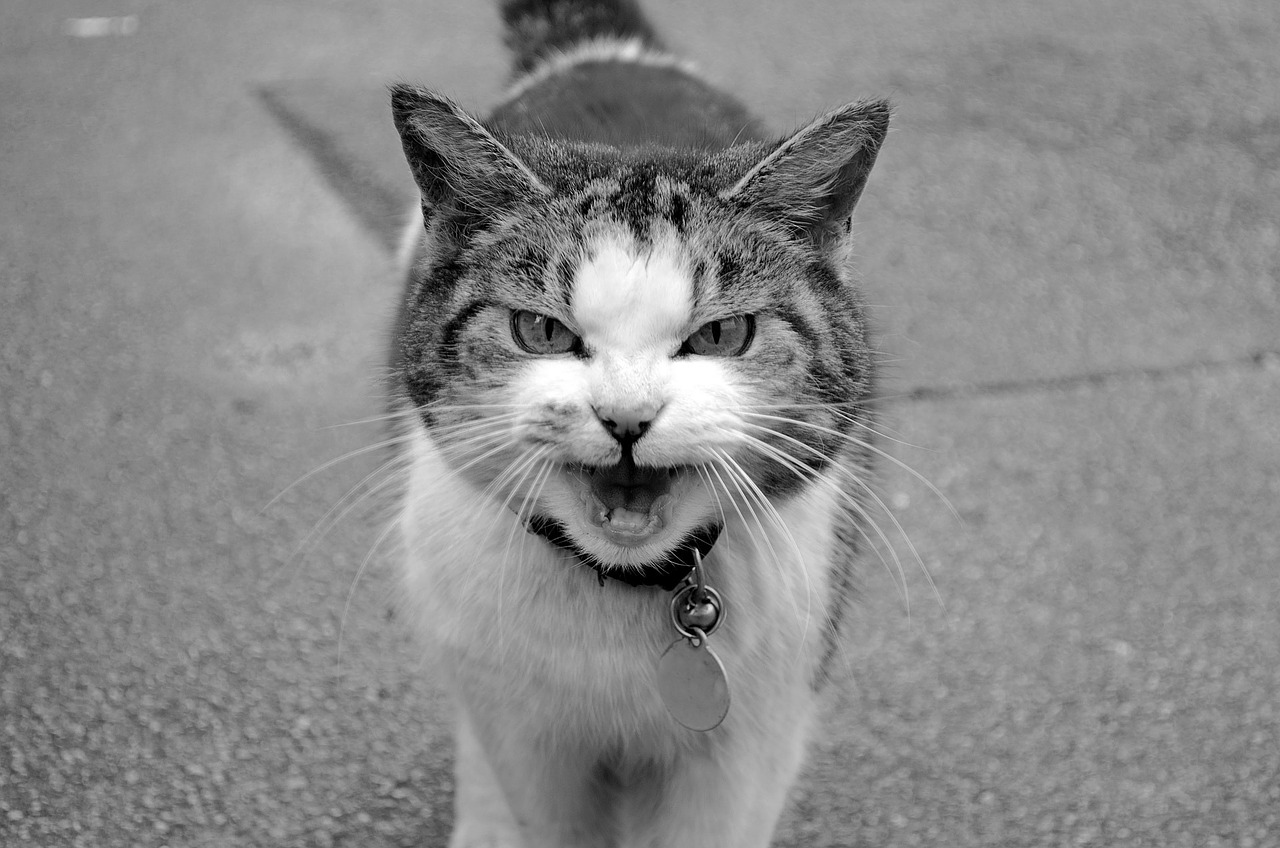
\includegraphics[width=0.99\textwidth]{bossycat}
                 \caption{Bossy} \label{fig2:bossycat}
         \end{subfigure}%
         \begin{subfigure}[b]{0.4\textwidth}
                 \flushright
                 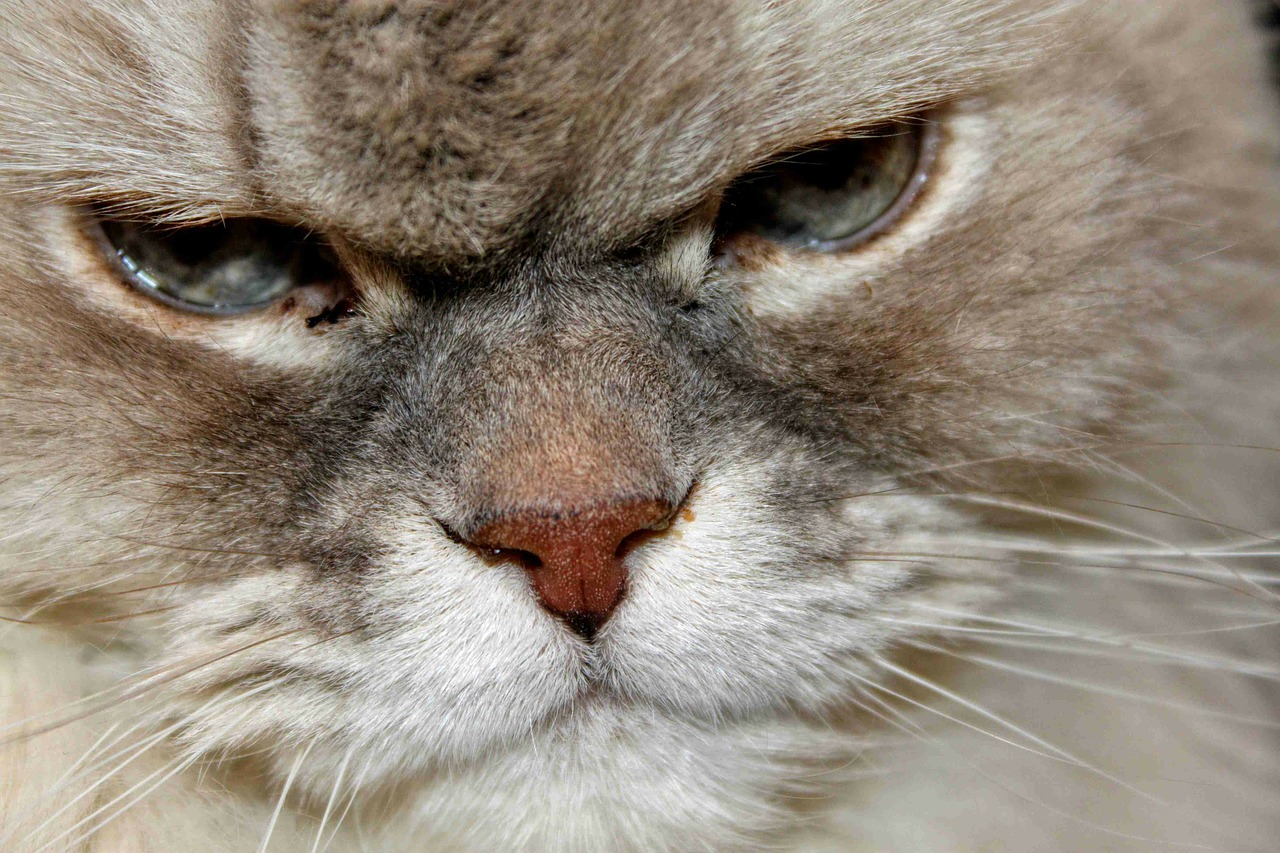
\includegraphics[width=0.98\textwidth]{frowningcat}
                 \caption{Reflective} \label{fig2:frowningcat}
         \end{subfigure}
% leave a blank line to change row         
         
         \begin{subfigure}[b]{0.31\textwidth}
                 \centering
                 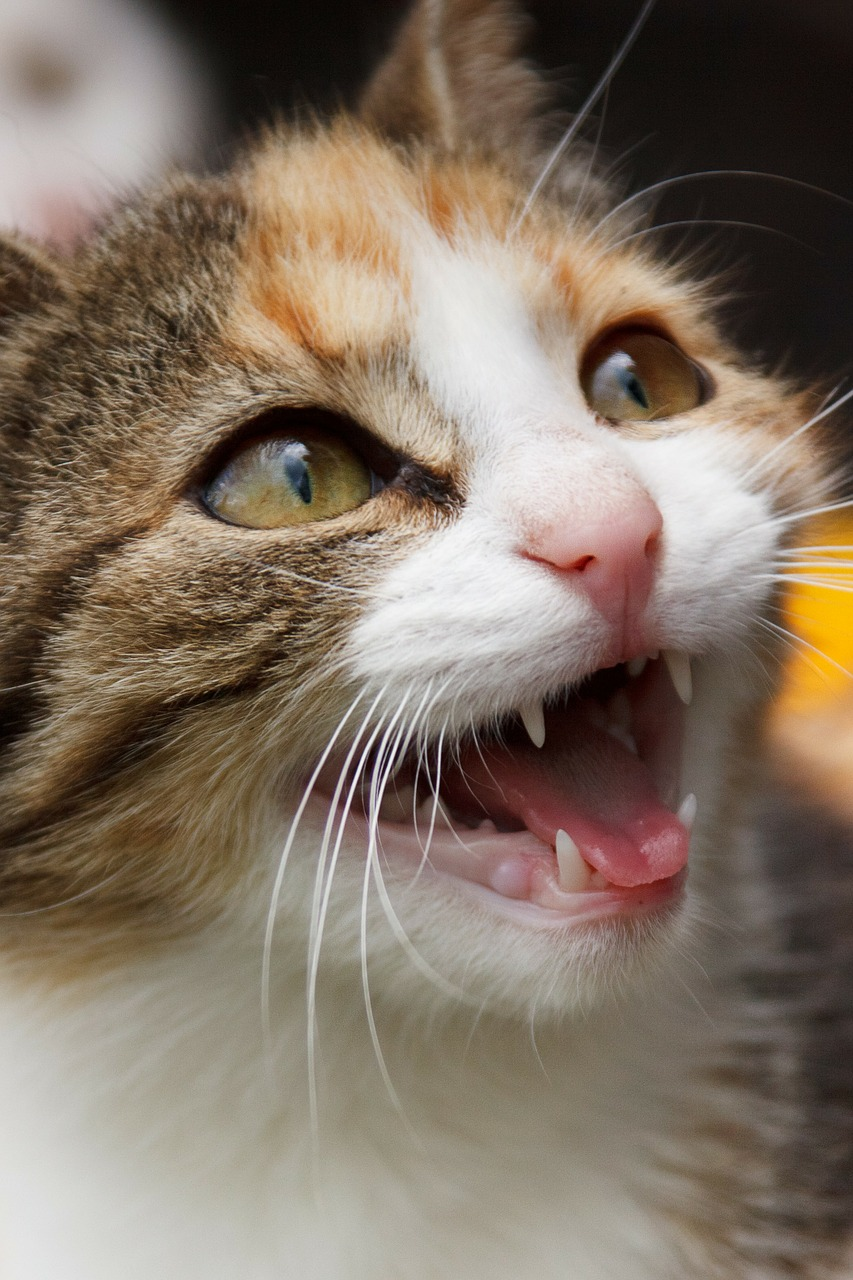
\includegraphics[width=0.985\textwidth]{scaredbabycat}
                 \caption{Scared} \label{fig2:scared}
         \end{subfigure}
         \begin{subfigure}[b]{0.69\textwidth}
                 \centering
                 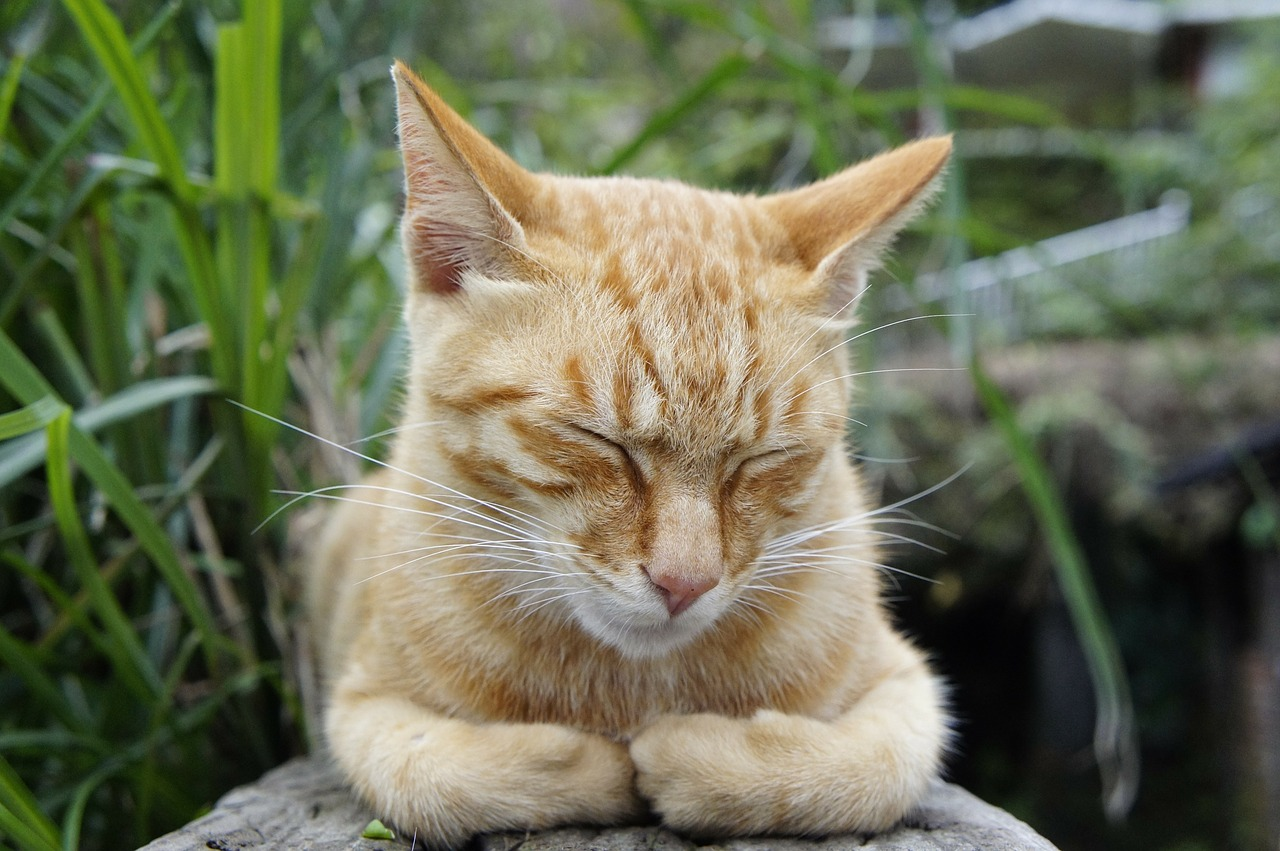
\includegraphics[width=\textwidth]{tiredcat}
                 \caption{Tired} \label{fig2:tired}
         \end{subfigure}
\begin{tablenotes}
\item Images in the public domain.
\end{tablenotes}
\end{cmpfigure}
\end{verbatim}
}

\clearpage
\section{Gantt chart} \label{ApB}
\begin{cmpfigure}[htb]{Project Gantt chart \label{pplan}}
\begin{sideways}
\newganttchartelement{voidbar}{
voidbar/.style={
draw=black,
top color=black!25,
bottom color=black!23
}}
\begin{ganttchart}[x unit=0.35cm, y unit chart = 1.0cm, y unit title=0.5cm, title height=1.0, vgrid, title label font=\scriptsize,
canvas/.style={draw=black, dotted},
/pgfgantt/milestone left shift = 0,
/pgfgantt/milestone right shift = 0
]{1}{34}
\gantttitle{Project schedule shown for semester week numbers}{34} \\
\gantttitlelist{1,...,34}{1}\\
\gantttitlelist{1,...,12}{1}
\gantttitle{CB}{4}
\gantttitle{AP}{2}
\gantttitlelist{1,...,8}{1}
\gantttitle{EB}{4}
\gantttitlelist{9,...,12}{1}\\
%the elements, bars and milestones, are identified as elem0, elem1, etc
%elem1
\ganttbar{Project proposal}{1}{2}     \\  %elem0  
\ganttbar{Literature review}{2}{5}    \\  %elem1 
\ganttbar{Design}{6}{11}              \\  %elem2
%week 1 of semester 2 is the 17th week in schedule 
\ganttbar{Coding}{12}{12}                 %elem3
\ganttvoidbar{}{13}{16}                   %elem4
\ganttbar{}{17}{20}                   \\  %elem5
\ganttbar{Testing}{12}{12}                %elem6
\ganttvoidbar{}{13}{16}                   %elem7
\ganttbar{}{17}{26}                    \\ %elem8
\ganttmilestone{Code delivery}{26}    \\ %elem9
\ganttbar{Final report writing}{25}{30}        \\ %elem10
\ganttmilestone{Portfolio submission}{33}  \\ %elem11
\ganttbar{Inspection prep}{31}{34}  %elem12
%
\ganttlink{elem0}{elem2} \ganttlink{elem1}{elem2} \ganttlink{elem2}{elem3}
\ganttlink[link mid=.25]{elem2}{elem6} \ganttlink{elem5}{elem6}
\ganttlink{elem8}{elem9} \ganttlink{elem9}{elem10}
\ganttlink{elem10}{elem11} \ganttlink{elem11}{elem12}
\end{ganttchart}
\end{sideways}
\end{cmpfigure}

\end{document}

